\subsubsection{The challenges performing Intra-Process Communication}\label{sec:ipc}
Ulemper ved at implementere IPC med mutex\footnote{Mere om mutexes, se afsnit~\ref{sec:mutex}.} og conditional\footnote{Conditionals i samspil med mutexes, se afsnit~\ref{sec:mtxcond}.} variable, eller semephore\footnote{Semaphore, se afsnit~\ref{sec:semaphore}.}.

\begin{itemize}
	\item Det er en udfordring at undgå deadlocks\footnote{Mere i afsnit~\ref{sec:deadlock}.} og timing issues (race conditions).\todo{link til forklaring af raceconditions.}
	\item Programmer bliver svære at læse og gennemskue (readability).
	\item Hvis en tråd venter på en bestemt betingelse (fx. condition variable), så laver den ikke noget fornuftigt i mellemtiden.
	\item Hvis tråde deler ressourcer:
	\begin{itemize}
		\item Rækkefølgen hvori de tager/låser ressourcen skal planlægges grundigt for at undgå deadlocks.
		\item Der skal muligvis låses flere mutexes, hvilket kan være meget tidskrævende.\todo{hvor tidskrævende er det at låse en mutex?}
	\end{itemize}
\end{itemize}

Optimalt vil vi forsøge at lave en løsning hvor følgende gælder:

\begin{itemize}
	\item Processering i en tråd kræver ikke noget lås (mutex etc). 
	\item Tråde kan kommunikere med hinanden.
	\item Kommunikation mellem tråde skal kunne indeholde data.
	\item Tråde skal kunne sende disse beskeder når de vil. De skal altså ikke være bundet af noget bestemt flow i programmet.
	\item Mange tråde kan kommunikere med flere andre tråde.\\
	\item Event-drevet programmering!.\todo{har andreas skrevet, men kan ikke lige se hvad det laver her?} 
\end{itemize}

\subsubsection{Message queue}
Disse beskedkøer skal fungere som ''mellemstation'' hvor besked kan opbevares før tråden er klar til at håndtere beskeden. Brugte vi ikke en sådan mekanisme ville beskeden ''gå tabt''. Alternativt skal vi bruge ressourcer på at synkronisere den sendende og modtagende part, således at beskeden sendes og modtages på ''samme tid''.

\todo{lav en short caption til dining phin.kjoij.}

\begin{itemize}
	\item FIFO kø, eventuelt med max på antal beskeder.
	\item Implementeret med STL \textit{queue}.
	\item Forskellige implementeringer:
	\begin{itemize}
		\item Asynkrone køer:
		\begin{itemize}
			\item Modtageren skal ikke have svar med det samme.
			\item I sekvensdiagrammet tegnes besked som en åben pil. \todo{indsæt ref til billede med eksempel} 
			\item Afsenderen kan forsætte operationer uden svar fra modtager.
		\end{itemize}
		\item Synkrone køer:
		\begin{itemize}
			\item Modtageren skal have svar med det samme.\todo{står den og venter? sover?}.
			\item I sekvensdiagrammet tegnes besked som en lukket pil. \todo{ref til eksempel}
			\item Afsenderen afventer svar fra modtageren før den kan forsætte operation.
		\end{itemize}
	\end{itemize}
\end{itemize}

\paragraph{The premises for designing it}

\paragraph{Various design solutions - Which one chosen and why}

\paragraph{Its design and implementation}

\subsubsection{Impact on design/implementation between before and after the Message Queue}

\subsubsection{Event Driven Programming}

\paragraph{Basic idea}
Event drevet programmering er opgjort af event producenter og event subscribers.
Tråde reagerer på indkommende events, og sover når der ikke sker noget.
Event drevet programmeret er specielt egnet til GUI applikationer hvor user inputs ofte bruges. \\

Der er flere måder at implementere EDP på. I vores ISU øvelse har vi brugt en MessageQueue hvis funktionalitet er beskrevet ovenfor.
Hvis vi ser på figur~\ref{fig:handlPat} vil vores MessageQueue være være mellemledet før dispatcheren. Det<e er smart da det ikke er sikkert at \textit{dispatcher} kan nå at videresende alle events til deres respektive handlers. MessageQueue'en fungerer derfor som en buffer.

\begin{figure}[h]
	\centering
	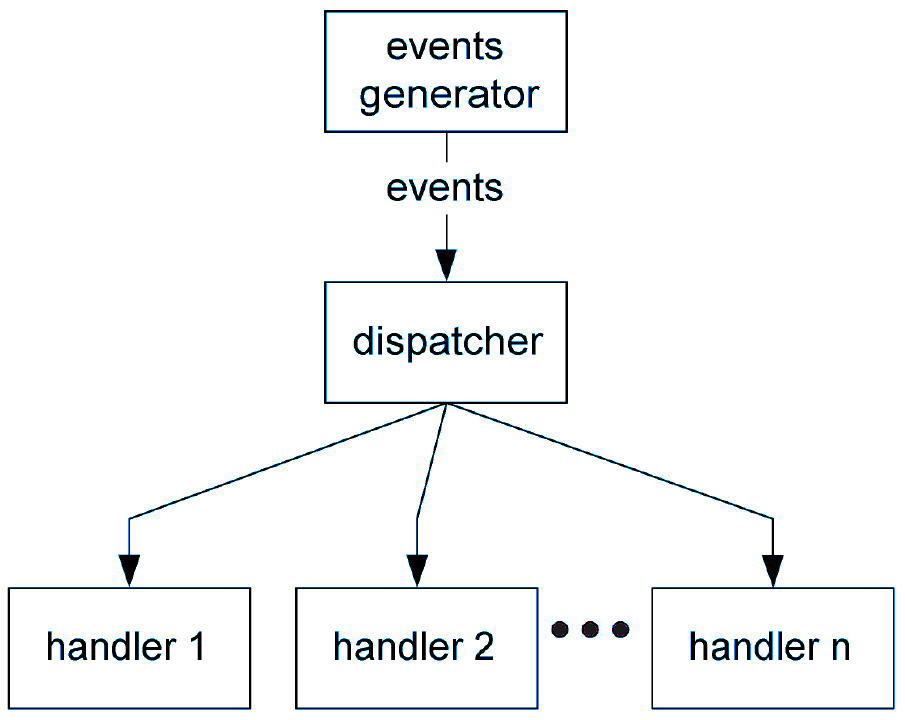
\includegraphics[width=0.6\linewidth]{figs/spm3/handlersPattern}
	\caption{Illustration af et handler pattern.}
	\label{fig:handlPat}
\end{figure}

Implementering kommer derfor til at følge dette mønster:

\begin{itemize}
	\item Genereing af beskeden?? \todo{skal man ikke det??}
	\item Get message fra MsgQueue.
	\item Kør dispatch.
	\item Handle event.
	\item De-alloker besked.
\end{itemize}

\paragraph{Reactiveness}

\paragraph{Design - e.g. from sequence diagrams to code (or vice versa)}
